
\chapter{$\varepsilon$-次模逼近网络的影响力最大化}

在$\varepsilon$-次模逼近网络中,一些节点的阈值函数是$\varepsilon$-次模逼近而不再是次模函数,整体的影响力函数也不再有次模性质。
本章中会先讨论$\varepsilon$-次模逼近节点的个数是图节点个数多项式的时影响力最大化的不可近似性,
然后又设计了$\varepsilon$-次模逼近节点较少时的近似算法。

\section{$(\gamma,\varepsilon)$-ASIM的不可近似性}
本节我们会证明对于$n$个节点的图中,即使只有有$n$的多项式个$\varepsilon$-次模节点,
影响力最大化问题也很难近似。
下文用定理给出这个不可近似性的精确描述,然后本节接下来的部分会证明这个定理。


\subsection{不可近似性的主要结论}
\begin{theorem}
\label{the:inapp}
对于任意的$\varepsilon \in (0,1)$和任意的$\gamma \in (0,1)$,
在$(\gamma,\varepsilon)$-次模逼近图上不存在近似比为$1 / n^{\frac{\gamma}{c}}$的影响力最大化近似算法,
除非P=NP,这里$c = 3+3/\log{\frac{2}{2-\varepsilon}}$。
\end{theorem}

这个定理说明了只要图中有$n^{\gamma}$个$\varepsilon$-次模节点,不管$\gamma$有多少,影响力最大化问题都不能被近似。
不可近似的程度正比于$\gamma$的大小,$\gamma$越大,影响力最大化问题越难被近似。
定力的证明基于机关(gadget)的构造,我们通过二叉树级联机关构造出一个概率与门(probabilistic-AND gate),
然后我们通过NP完全问题Set Cover的规约证明了不可近似比的下界。

\subsection{基于二叉树的概率与门}
本小节介绍概率与门的构造和计算与门成功的概率。先介绍基础的机关,然后介绍通过二叉树级联得到的概率与门,最后计算与门的概率。


\begin{figure}[htbp]
\centering
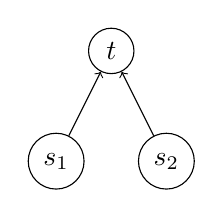
\begin{tikzpicture}[scale=0.7]
%\tikzstyle[thick]
\node at (1,2) [circle,draw](1) {$t$};
\node at (0,0) [circle,draw](2) {$s_1$};
\node at (2,0) [circle,draw](3) {$s_2$};
\path [->] (2) edge node{} (1);
\path [->] (3) edge node{} (1);
\end{tikzpicture}
\caption{基础机关结构}
\label{fig:gadget_basic}
\end{figure}
我们构建的机关如图\ref{fig:gadget_basic}所示,这个机关以节点$s_1,s_2$作为输入,以节点$t$作为输出。
节点$t$有两个入邻居,阈值函数$g(\cdot)$是$\varepsilon$-次模函数。
阈值函数$g(\cdot)$的赋值见等式\ref{eq:func_g}。
\begin{eqnarray*}
\label{eq:func_g}
g(S) =
\left\lbrace
\begin{aligned}
&0,		~ & |S|=0; \\
&\frac{1-\varepsilon}{2},	~ & |S|=1; \\
&1,		~ & |S|=2. \\
\end{aligned}
\right.
\end{eqnarray*}
函数$g(S)$的取值只依赖于输入集合的大小$|S|$,$g(\cdot)$被夹在两个线性的次模函数之间。
$g(\cdot)$自身是一个线性函数在$|S|=1$处向下偏移了$\varepsilon$。
这个基础机关距离与门的性质还很远,接下来我们介绍如何构造更复杂的机关。


我们希望构建出一个机关满足如下性质:
\begin{eqnarray*}
P_a(t) =
\left\lbrace
\begin{aligned}
&1,		~ & \mbox{$s_1,s_2$均被激活}; \\
&o(1),	~ & \mbox{$s_1,s_2$中只有一个被激活}; \\
&0,		~ & \mbox{$s_1,s_2$都未被激活}. \\
\end{aligned}
\right.
\end{eqnarray*}
其中$P_a(t)$是机关的输出节点$t$被激活的概率。
满足这样的性质,当输入节点$s_1,s_2$没有被全部激活时,输出节点$t$很大概率不会被激活。
前面的基础机关在$|S|=1$时,$t$被被激活的概率是$\frac{1-\varepsilon}{2}$,
我们做的就是通过二叉树级联机关放大$\frac{1-\varepsilon}{2}$和$\frac{1}{2}$的差距,
最终使得$|S|=1$时$t$很大概率不被激活,机关的构造如图\ref{fig:gadget_tree}所示。


\begin{figure}[htbp]
\centering
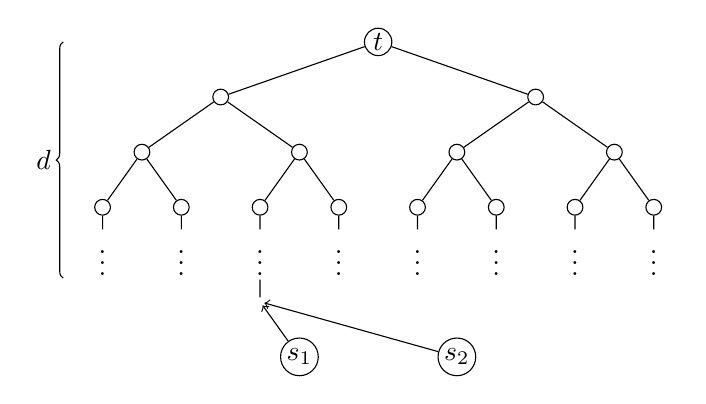
\begin{tikzpicture}[every node/.style={draw,circle,inner sep=1pt}]
% \draw[step=1cm, color=gray] (-5,-5) grid (5,5);
\tikzstyle{level 1}=[sibling distance=40mm,level distance=7mm]
\tikzstyle{level 2}=[sibling distance=20mm]
\tikzstyle{level 3}=[sibling distance=10mm]
\tikzstyle{level 4}=[level distance=6mm]
%\tikzstyle{level 5}=[sibling distance=15mm,level distance=10mm]
\draw[decorate, decoration={brace, mirror}] (-4cm, 0) -- (-4cm,-3cm);
\draw (-4.25cm, -1.5cm) node[draw=none] {$d$};

\node at (-1,-4) [circle,draw](2) {$s_1$};
\node at (1,-4) [circle,draw](3) {$s_2$};
\node {$t$}
	child{
		node{$~$}
		child{
			node{$~$}
			child{
				node{$~$}
				child{node[draw=none] {$\vdots$}
				}
			}
			child{
				node{$~$}
				child{node[draw=none]{$\vdots$}}
			}
		}
		child{
			node{$~$}
			child{
				node{$~$}
				child{node[draw=none]{$\vdots$}
					child{node[draw=none] (leaf_1) {$ $}}
				}
			}
			child{
				node{$~$}
				child{node[draw=none]{$\vdots$}
				}
			}
		}
	}
	child{
		node{$~$}
		child{
			node{$~$}
			child{
				node{$~$}
				child{node[draw=none]{$\vdots$}
				}
			}
			child{
				node{$~$}
				child{node[draw=none]{$\vdots$}}
			}
		}
		child{
			node{$~$}
			child{
				node{$~$}
				child{node[draw=none]{$\vdots$} }
			}
			child{
				node{$~$}
				child{node[draw=none] {$\vdots$}
					%child{node[draw=none] (leaf_2) {$ $}}
				}
			}
		}
	};

\path [->] (2) edge (leaf_1);
\path [->] (3) edge (leaf_1);
\end{tikzpicture}
\caption{二叉树机关$T_\varepsilon$}
\label{fig:gadget_tree}
\end{figure}

在这棵满二叉树中,输出节点$t$是二叉树的根节点,每个节点有一条有向边指向它的父节点。
对每个叶子结点$v$,输入节点$s_1,s_2$会发出有向边指向$v$。
二叉树中每个节点的阈值函数都是前文等式\ref{eq:func_g}定义的$\varepsilon$-次模函数$g(\cdot)$。
整个树状结构被定义为$T_\varepsilon$,$\varepsilon$就是函数$g(\cdot)$距离次模函数的偏移量。
二叉树的深度会在后文定义,我们用$v_i$表示深度为$i$的节点($t$的深度是$1$)。


很显然$s_1,s_2$都被激活时$P_a(t)=1$,$s_1$ or $s_2$都没有被激活时$P_a(t)=0$。
下面我们证明对于深度$d$的二叉树,$s_1,s_2$中只有一个被激活时,输出节点$t$被激活的概率是$O(2^{-d})$。
\begin{lemma}
\label{lem:tree_prob}
对于深度为$d$的机关$T_\varepsilon$,当输入节点只有一个被激活时,
输出节点$t$被激活的概率小于$(\frac{2-\varepsilon}{2})^{d}$。
\end{lemma}
\begin{proof}
对于所有的叶子结点$v_d$,可以得到$P_a(v_d) = \frac{1-\varepsilon}{2}$。
机关$T_\varepsilon$中同一层的节点之前激活与否是互相独立的。
给定一个基础机关(如图\ref{fig:gadget_basic}),如果每个输出节点被激活的概率都是$p$而且互相独立,则输出节点$t$被激活的概率是
\begin{equation*}
\begin{array}{ll}
& P_a(t) \\
= & p^2\times g(2) + 2p(1-p)\times g(1) + (1-p)^2\times g(0) \\
= & p^2 + 2p(1-p)\frac{1-\varepsilon}{2} = p(1-\varepsilon(1-p)).
\end{array}
\end{equation*}
根据这个公式,我们可以写出二叉树上不同深度节点被激活概率的递推公式。
\begin{equation}
\label{eq:recurrence}
P_a(v_i) = P_a(v_{i+1})(1-\varepsilon(1-P_a(v_{i+1}))) <  P_a(v_{i+1})(1-\varepsilon/2)
\end{equation}
不等号的成立是因为树的叶节点满足$P_a(v_d) = \frac{1-\varepsilon}{2}$,而且随着节点所处深度降低,被激活的概率递减。
所以对于树中的任意节点$v$都有$P_a(v) < \frac{1}{2}$。
根据递推公式\ref{eq:recurrence},输出节点$t$被激活的概率为
\begin{equation*}
\label{eq:p_a_t}
 P_a(t) 
=  P_a(v_1) 
<  \frac{1-\varepsilon}{2}(\frac{2-\varepsilon}{2})^{d-1} 
<  (\frac{2-\varepsilon}{2})^{d}.
\end{equation*}
节点$t$被激活的概率$P_a(t) = O(2^{-d})$,随着$d$的增加趋于$0$。
\end{proof}
由引理\ref{lem:tree_prob}我们知道$T_\varepsilon$在输入集合大小为$1$时输出节点被激活的概率是$o(1)$,
$T_\varepsilon$的确是一个概率与门。

先说m们,然后下一节说sketch
We then construct a multi-input probabilistic-AND gate based on our probabilistic-AND gate by the similar method to construct multi-input-AND gate based on 2-input-AND gate. Finally, we show if influence maximization problem can be approximated beyond the ratio shown above, we can solve the set cover problem in polynomial time. The main idea is as follows. For any set cover instance, we will put all elements to be the input of our multi-input-probabilistic-AND gate, and connect the output with a large number of additional nodes. Thus, if $k$ sets can cover all elements, all of those addition nodes will be activated, on contrast, if one of the elements cannot be covered, almost all of the additional nodes will remain inactivated.

\subsection{基于Set Cover的不可近似性规约}
在本节基于概率与门,我们证明定理\ref{the:inapp}。
\begin{proof}[定理\ref{the:inapp}]
We have described the construction of gadget $T_\varepsilon$, we can further construct $m$-input trees
$T_\varepsilon^m$ with gadget $T_\varepsilon$ --- a multi input AND gate.
Given $n$ input nodes $s_1, s_2, \dots, s_n$,
we can use $s_0$ and $s_1$ as input nodes of $T_\varepsilon$ and set output node as $s_{12}$.
And then combine $s_{12}$ and $s_{3}$ with gadget $T_\varepsilon$ to obtain output $s_{123}$.
Finally we obtain ultimate output node $s_{12\dots n}$.
We can say that $s_{12\dots n}$ can be activated only when all the nodes $s_1, s_2, \dots, s_n$ are activated,
if for all $T_\varepsilon$ node $t$ will not become activated when not all its input nodes are activated,
We calculate the probability that $T_\varepsilon^n$ is an AND gate.
Since each $T_\varepsilon$ is a binary tree with depth $d$,
each $T_\varepsilon$ breaks the AND gate rule with probability at most $(\frac{2-\varepsilon}{2})^{d}$.
With Union Bound, we can say that $T_\varepsilon^m$ is an AND gate with probability at least $1-n(\frac{2-\varepsilon}{2})^{d}$.
Besides, a $T_\varepsilon^n$ have $n\times(2^d-1) = n2^d-n$ nodes.

We consider a variant of set cover problems and show that if influence maximization problem can be approximated beyond the ratio shown above,
then we can solve the set cover problem.
Let $e_1, e_2, \dots, e_n$ denote the nodes corresponding to the $n$ elements.
Let $s_1, s_2, \dots, s_m$ denote the nodes corresponding to the $m$ sets.
We can assume that $m<n$.
When $m\geq n$ we could add $m$ dummy nodes that contained by all $m$ sets,
the solution of the newly created graph is the same with original graph.
Each set node $s_i$ holds a directed edge towards the element nodes it covers
and each element node $e_i$ has threshold function with $f_{e_i}(1)=1$,
which means that $e_i$ becomes activated when at least one of the nodes corresponding to to sets covering it is activated.
We further add $n^\alpha$ nodes named $x_1, x_2, \dots, x_{n^\alpha}$, where $\alpha$ is a large positive constant.
Each node $x_i$ is the output of a $T_\varepsilon^n$ and $e_1, e_2, \dots, e_n$ are the input nodes.
Besides, for a large positive constant $\alpha$,
we add $n^\beta$ children $c_1, c_2, \dots, c_{n^\beta}$ for each node $x_i$.
Each child node $c_i$ also has threshold function with $f_{c_i}(1)=1$.
Here we calculate the depth of $T_\varepsilon$ in order to make sure that the $n^\alpha$ $T_\varepsilon^n$ are all AND gate with high probability.
Again we apply Union Bound to calculate the probability upper bound of at least one $T_\varepsilon^n$ fails
--- $n^{1+\alpha}(\frac{2-\varepsilon}{2})^{d}$.
We set $d = (1+\alpha+\lambda)\log n / \log{\frac{2}{2-\varepsilon}}$,
so all the $T_\varepsilon^n$ observe the rule of AND gate with probability at least $1-n^{-\lambda}$.

If we can find $k$ sets that cover all the $n$ elements, then we just select the $k$ nodes corresponding to the $k$ sets as seed nodes.
Then the seed nodes will activate nodes $e_1, e_2, \dots, e_n$ and then all nodes in gadgets $T_\varepsilon^n$ will become activated.
Finally, all the child nodes of $x_1, x_2, \dots, x_{n^\alpha}$ become activated, and totally $k+n+n^{\alpha+1}(2^d-1)+n^{\alpha\beta} \geq n^{\alpha\beta}$ nodes become activated in total, while the graph consists of $N = m+n+n^{\alpha+1}(2^d-1)+n^{\alpha\beta}$ nodes, nearly all nodes are activated.
On the other hand, if there is no solution of size $k$ for this set cover problem, we can not activate all element nodes $e_i$.
During the influence spread of a given target nodes,
none of $x_1, x_2, \dots, x_{n^\alpha}$ will become activated with probability al least $1-n^{-\lambda}$.
Under this circumstance, we can select nodes labeled with $x$ as seeds or just try to activate more nodes $e_i$.
Totally we can just activate at most $k+n+kn^{\beta}$ nodes if we choose $x_i$ as seeds.
Otherwise we can assume that at most $n-1$ elements are covered and all gadget nodes are activated.
In this case $k+n-1+n^{\alpha+1}(2^d-1)$ nodes will become active if all probabilistic AND gate work perfectly.
One the other hand if these $T_\varepsilon^n$ fails with probability at most $n^{-\lambda}$, we just assume that all the nodes will become activated eventually.
We can set $n^{\beta} = n^{\alpha-1} \cdot 2^d \cdot n^{\delta}$ for $\delta>0$ to 
ensure that the fraction of gadget nodes and dummy nodes is slightly less than $n^{\frac{1}{\alpha-1}}$. 
When $n$ is large enough the influence size we obtain  
is less then $kn^{\beta} \leq n^{\beta+1}$ or $n^{\alpha+1}2^d$ w.h.p. when Set Cover is not solved.
For any influence maximization algorithm,
there exists a graph of $N$ nodes where at most $n^{\alpha+1}(2^d-1)$ nodes have $\varepsilon$-almost submodular threshold function,
for any result obtained,
with probability at least $1-n^{-\lambda}$,
the influence size is less than $1/n^{\alpha-1}$ of $\sigma(S^*)$,
unless we can solve Set Cover problems within polynomial time.
Here $N \geq n^{\alpha+\beta}$, $d = (1+\alpha+\lambda)\log n / \log{\frac{2}{2-\varepsilon}}$, $\beta = (\alpha+1) + (1+\alpha+\lambda) / \log{\frac{2}{2-\varepsilon}} + \delta$.
We can substitute the parameter into the conclusion, we obtain that $\forall \alpha>1, \lambda>0, \delta>0$, there exists
$b = 1/\log{\frac{2}{2-\varepsilon}}$,
$\varphi= \frac{ \min\{\alpha-1, \lambda\}}{2\alpha+\delta-1+b(1+\alpha+\lambda)}$ and
$\gamma =\frac{\alpha+1+b(1+\alpha+\lambda)}{2\alpha+\delta-1+b(1+\alpha+\lambda)}$,
for any influence maximization algorithm based on measg{gamma},
there exists an instance of graph,
the approximation ratio is less than $n^{-\gamma}$.
Notice that $\varphi \geq \frac{\gamma}{3+3b}$ when we set $\alpha=\lambda+1$ and $\lambda \geq 1$.
$\gamma$ ranges in $(0,1)$, hence the theorem follows.
\end{proof}

\section{近似算法}


\section{本章小结}








